\documentclass[../linear-spaces.tex]{subfiles}

\begin{document}
\chapter{Projections onto subspaces}

A projection is an idempotent mapping of a set (or any structure) into a subset
(or sub-structure). Idempotent means that, projecting once is the same as
projecting $n$-times.

We will see this as a vector being projected in a line, a line is a subspace of
$\mathbb{R}$, and our vector is in $\mathbb{R}^{2}$.

\begin{center}
    \begin{tikzpicture}
        \coordinate (v) at (2,3);
        \coordinate (e) at (14/5, 7/5);
        \coordinate (l1) at (-2,-1);
        \coordinate (l2) at (4,2);

        \draw[thick, dashed] (l1)--(l2);
        \draw[->, thick] (0,0)--(0,5);
        \draw[->, thick] (0,0)--(5,0);
        \draw[->, very thick] (0,0)--(v);
        \draw[dashed] (v)--(e);
        \draw[->, very thick] (0,0)--(e);

        \draw (l2) + (0.2,0.2) node{$l$};
        \draw (e) + (0, 1) node{$e$};
        \draw (v) + (-1, -1) node{$v$};
        \draw (e) + (-.9, -.9) node{$proj_u {v}$};

    \end{tikzpicture}
\end{center}

This is the most basic example of projection. Let's deduce a formula.

\begin{example}
    Let $v\in\mathbb{R}^{2}$ and let $l$ be a line
    in $\mathbb{R}^{2}$ parametrized by a vector $u$ as $f(t)=ut$.

    \begin{center}
        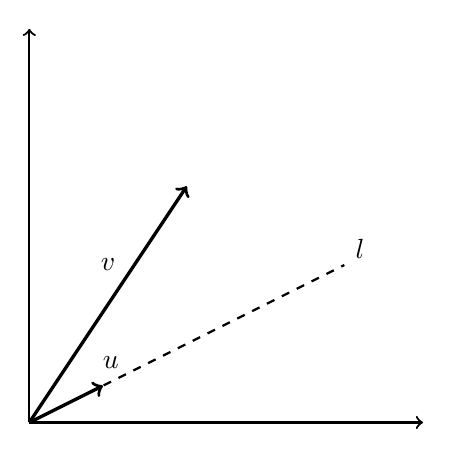
\begin{tikzpicture}
            \coordinate (v) at (2,3);
            \coordinate (e) at (14/15, 7/15);
            \coordinate (l1) at (0,0);
            \coordinate (l2) at (4,2);

            \draw[thick, dashed] (l1)--(l2);
            \draw[->, thick] (0,0)--(0,5);
            \draw[->, thick] (0,0)--(5,0);
            \draw[->, very thick] (0,0)--(v);
            \draw[->, very thick] (0,0)--(e);

            \draw (l2) + (0.2,0.2) node{$l$};
            \draw (v) + (-1, -1) node{$v$};
            \draw (e) + (.1,.3) node{$u$};

        \end{tikzpicture}
    \end{center}

    What we want to find is some constant $k$ such that $ku$ is perpendicular to
    $l$. We know from the previous image that $e=proj_u v - v = uk-v$

    \begin{equation*}
        \begin{split}
            (ku-v)\cdot u = k\|u\|^{2} - v\cdot u = 0
        \end{split}
    \end{equation*}

    Then $k=\frac{v\cdot u}{\|u\|^{2}}$. The formula for projection becomes

    \begin{equation}
        \begin{split}
            proj_u v = ku = \frac{v\cdot u}{\|u\|^{2}}\cdot u
        \end{split}
    \end{equation}

    We call this projection in terms of $u$, because $l$ is parametrized by $u$.
\end{example}

Now, we want to extend this idea to any linear space. We can see that a
projection is a multiplication of the ``projection basis'' by some scalar.

This gives us an idea of what the inner product is: we can think of the inner
product as ``how much of some element is onto other element''. Think of
projecting a vector $v$ onto $u$ when $v\perp u$.

\begin{center}
    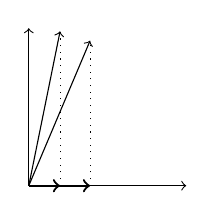
\begin{tikzpicture}
        \coordinate (v) at (2,0);
        \coordinate (e) at (0,2);
        \coordinate (c) at (0.778836684617, 1.84212198801);
        \coordinate (d) at (0.39733866159, 1.96013315568);

        \draw[->] (0,0)--(v);
        \draw[->] (0,0)--(e);
        \draw[->] (0,0)--(c);
        \draw[->] (0,0)--(d);
        \draw[dotted] (0.39733866159,0) -- (d);
        \draw[dotted] (0.778836684617,0) -- (c);
        \draw[->, thick] (0,0) -- (0.778836684617,0);
        \draw[->, thick] (0,0) -- (0.39733866159,0);
    \end{tikzpicture}
\end{center}

You can see that the projection tends to a vector with no length. This can be
proven easily with (2.2):

\begin{equation}
    \begin{split}
        proj_u v = u\cdot\frac{u\cdot v}{\|u\|^{2}}
        \\ = u\cdot\frac{\|v\|}{\|u\|} \cos\psi
    \end{split}
\end{equation}

The $\frac{\|v\|}{\|u\|}$ part is the amount of times $u$ fits in $v$, and if
$\psi = \frac{\pi}{2}$ then the projection is the $O$ vector.

\begin{example}[Projections in $\mathbb{R}^{n}$]
    Let $x\in\mathbb{R}^{n}$ be a vector in a plane, this plane must be of dimension $n-1$.
    Thus, it has a basis with $n-1$ elements given by
    \begin{equation*}
        W = \left(e_1, e_2,\dots, e_{n-1}\right)
    \end{equation*}

    Where $e_1,e_2,\dots,e_{n-1}\in\mathbb{R}^{n}$. These vectors parametrize the
    plane, such that $x$ can be written as
    \begin{equation}
        \begin{split}
            x = \sum_{i=1}^{n-1}{c_i e_i}
        \end{split}
    \end{equation}

    for any scalars $c_1,c_2,\dots,c_{n-1}$. Now, suppose that we have a vector
    $v\in\mathbb{R}^{n}$ that preferably, does not lie in this plane.

    To find the projection, we can set a set of equation that are analogous to the
    example in $\mathbb{R}^{2}$:
    \begin{equation}
        \begin{split}
            \begin{cases}
                e_1(v - k x) = 0 \\
                e_2(v - k x) = 0 \\
                \cdots           \\
                e_{n-1}(v - k x) = 0
            \end{cases}
        \end{split}
    \end{equation}

    Where $k\in\mathbb{R}$. What we want is to make each basis vector orthogonal to
    a vector $x$ that connects $v$ to the plane. In other words, the vector
    $(v-kx)$ will be perpendicular to the plane.

    We will collect each basis vector into a matrix
    \begin{equation}
        A = \left[
            \begin{matrix}
                \vdots & \vdots &        & \vdots  \\
                e_1    & e_2    & \cdots & e_{n-1} \\
                \vdots & \vdots &        & \vdots  \\
            \end{matrix}
            \right]
    \end{equation}

    Here, $A$ has dimension $n\times (n-1)$. The system of equations in (3.4)
    becomes
    \begin{equation}
        A^{T}\left(v-kx\right) = 0
    \end{equation}

    But we can rewrite $x$ as a vector $c$ times $A$, so that
    \begin{equation}
        x = Ac =  \left[\begin{matrix}
                \vdots & \vdots &        & \vdots  \\
                e_1    & e_2    & \cdots & e_{n-1} \\
                \vdots & \vdots &        & \vdots  \\
            \end{matrix}\right]\cdot\left[\begin{matrix}
                c_1 \\c_2\\\vdots\\c_{n-1}
            \end{matrix}\right]
    \end{equation}

    You can verify that this is the same as writing $x$ in the form (3.3).
    Rewriting equation (3.6) leaves
    \begin{equation*}
        A^{T}\left(v-Ac\right) = 0
    \end{equation*}

    We omit the term $k$ since we will assume that the vector $c$ scales $x$
    accordingly. Expanding the equation
    \begin{equation}
        \begin{split}
            A^{T}\left(v-Ac\right) = A^{T}v - A^{T}Ac = 0
        \end{split}
    \end{equation}

    Now, we solve for $c$
    \begin{equation}
        \begin{split}
            c={(A^{T}A)}^{-1}A^{T}v
        \end{split}
    \end{equation}

    Now, as the projection is given by scaling all the basis vectors in $A$ by $c$
    (think of $c$ as the scalar term in the 2-dimensional example), we can write
    our projection vector $p$ as

    \begin{equation}
        p = Ac = A{(A^{T}A)}^{-1}A^{T}v = Pv
    \end{equation}

    We define $P$ to be the \textbf{projection matrix}, and $v$ is the vector
    projected onto the plane $A$.

    To figure out the equation of the plane, we think of the definition of a plane:
    each vector in the plane must be perpendicular to a normal vector. This means
    that we always have $A\cdot n = O$, where $n$ is the normal vector.

    We can write the equation for an hyperplane in $\mathbb{R}^{n-1}$ as
    \begin{equation}
        n^{T}(x-x_0) = 0
    \end{equation}

    where:
    \begin{itemize}
        \item $n \in \mathbb{R}^n$ is the \textbf{normal vector} to the hyperplane,
        \item $x \in \mathbb{R}^n$ is any point \textbf{on} the hyperplane,
        \item $x_0 \in \mathbb{R}^n$ is a fixed point in the hyperplane (used to position or ``anchor'' the hyperplane in space).
    \end{itemize}

    This equation states that the vector from $x_0$ to any point $x$ on the
    hyperplane is \textbf{orthogonal} to the normal vector $n$, ensuring all such
    points lie in the same flat $(n-1)$-dimensional space.

    In this definition we didn't use the basis vectors in $W$, however as $x$ is a
    combination of basis vectors, it is not necessary to explicitly write them.
\end{example}

Some important applications of projections are \textbf{linear regression}, or
the \textbf{Fourier series} we will see how to derive them later.

% TODO: Fourier series %

\begin{example}[Linear Regression]
    Let $S$ be a set of points in $\mathbb{R}^{n-1}$, suppose we can map the points
    with a scalar field given by $f:\mathbb{R}^{n-1}\to\mathbb{R}$, this means that
    $S$ can be written as:
    \begin{equation}
        \begin{split}
            S = \left\{\left(x_{11},x_{12},\dots,x_{1(n-1)},z_{1} \right), \dots, \left(x_{m1}, x_{m2},\dots,x_{m(n-1)}, z_m\right)\right\}
        \end{split}
    \end{equation}

    We can set a system of equations that uses a coefficient vector $u$ and a
    \textit{bias}:
    \begin{equation}
        \begin{cases}
             & x_{11}u_1 + x_{12}u_2 + \cdots + x_{1(n-1)}u_{n-1} + b = z_1
            \\                                                                                                                                                                                                             & x_{21}u_1 + x_{22}u_2 + \cdots + x_{2(n-1)}u_{n-1} + b = z_2
            \\                                                                                                                                                                                                             & \qquad \qquad \qquad \qquad \vdots
            \\ &x_{m1}u_1 + x_{m2}u_2 + \cdots + x_{m(n-1)}u_{n-1} + b = z_m
        \end{cases}
    \end{equation}

    Each $z$ is a combination of $n-1$ independent variables, plus a bias term. We
    can rewrite the system as an $m\times n$ matrix multiplied by an $n\times 1$
    vector
    \begin{equation}
        \left[
            \begin{matrix}
                1      & x_{11} & x_{12} & \cdots & x_{1(n-1)} \\
                1      & x_{21} & x_{22} & \cdots & x_{2(n-1)} \\
                \vdots & \vdots & \vdots & \ddots & \vdots     \\
                1      & x_{m1} & x_{m2} & \cdots & x_{m(n-1)} \\
            \end{matrix}
            \right]\cdot \left[
            \begin{matrix}
                b \\ u_1 \\\vdots\\u_{n-1}
            \end{matrix}
            \right] = \left[
            \begin{matrix}
                z_1 \\z_2\\\vdots\\z_m
            \end{matrix}
            \right]
    \end{equation}
    \begin{equation*}
        X\cdot u = z
    \end{equation*}

    We want to fit the equation to an approximation vector $\hat u$. The vector $z$
    lies in a hyperplane. $\hat u$ is essentially a vector that gives the direction
    of a line that fits these points at best. This works because, the projection
    gives the minimum distance to $z$.
    \begin{equation}
        \hat u = {\left(X^{T}X\right)}^{-1}X^{T}z
    \end{equation}

    But this approximation only has one dimension for the output. If you let $z$ be
    a matrix, so that each output of the system of equations is a vector, then
    define $u$ to be a $n\times p$ matrix and $z$ to be $m\times p$.
    \begin{equation}
        \left[
            \begin{matrix}
                1      & x_{11} & \cdots & x_{1(n-1)} \\
                1      & x_{21} & \cdots & x_{2(n-1)} \\
                \vdots & \vdots & \ddots & \vdots     \\
                1      & x_{m1} & \cdots & x_{m(n-1)} \\
            \end{matrix}
            \right]\cdot \left[
            \begin{matrix}
                b_1        & \cdots & b_p        \\
                u_{11}     & \cdots & u_{1p}     \\
                \vdots     & \ddots & \vdots     \\
                u_{(n-1)1} & \cdots & u_{(n-1)p} \\
            \end{matrix}
            \right] = \left[
            \begin{matrix}
                z_{11} & \cdots & z_{1p} \\
                z_{21} & \cdots & z_{2p} \\
                \vdots & \ddots & \vdots \\
                z_{m1} & \cdots & z_{mp} \\
            \end{matrix}
            \right]
    \end{equation}

    Then $\hat u$ has dimension $n \times p$, defining a hyperplane that best fits
    the data in $X$ across all output dimensions.

    While $\hat u$ provides an approximation for each point in $X$, the hyperplane
    must fit all points. In an $n$-dimensional space, this requires only $n$
    coefficients.

    For that, we can take the mean of each row (as we have $n$ rows) and
    approximate a plane with the following equation:
    \begin{equation}
        \begin{split}
            P(x_1, x_2, \dots, x_{n-1}) = \bar{b} + \bar{u}_1 x_1 + \cdots + \bar{u}_{n-1} x_{n-1}        \end{split}
    \end{equation} Where
    \begin{itemize}
        \item $\bar{b} = \dfrac{1}{p}\sum_{i=1}^{p}{b_i}$
        \item $\bar{u}_i = \dfrac{1}{p}\sum_{j=1}^{p}{u_{i j}}$ for $\,i\in\left\{1,2,\dots,n-1\right\}$
    \end{itemize}

    \textbf{Worked example: } Suppose that we have a set of points given in the table below:

    \begin{center}
        \begin{tabular}{|c|c|c|c|c|}
            \hline
            \textbf{Point} & $x_1$ & $x_2$ & $z^{(1)}$ & $z^{(2)}$ \\
            \hline
            1              & 2     & 3     & 10        & 11        \\
            2              & 6     & 7     & 9         & 8         \\
            3              & 4     & 2     & 7         & 9         \\
            \hline
        \end{tabular}
    \end{center}

    Note that we have two different outputs, namely $z^{(1)}$ and $z^{(2)}$. This
    is because we can have multiple readings for the same inputs $x_1,x_2$.

    Now, using the method described above we can set up our system of equations
    \begin{equation}
        \begin{split}
            X\cdot u = z \\[1em]
            \begin{bmatrix}
                1 & 2 & 3 \\
                1 & 6 & 7 \\
                1 & 4 & 2 \\
            \end{bmatrix}
            \cdot
            \begin{bmatrix}
                b_1    & b_2    \\
                u_{11} & u_{12} \\
                u_{21} & u_{22}
            \end{bmatrix}
            & =
            \begin{bmatrix}
                10 & 11 \\
                9  & 8  \\
                7  & 9  \\
            \end{bmatrix}
        \end{split}
    \end{equation}

    Solving for $\hat{u} = \left(X^{T}X\right)^{-1}X^{T}z$:
    \[
        \hat{u} =
        \begin{bmatrix}
            9.6667  & 12.3333 \\
            -1.0833 & -0.9167 \\
            0.8333  & 0.1667
        \end{bmatrix}
    \]

    Now, we take the mean of each row and convert it to a column vector $\bar{u}$
    \[
        \bar{u} = \left[
            \begin{matrix}
                \bar{b} \\\bar{u}_1\\\bar{u}_2
            \end{matrix}
            \right] = \left[
            \begin{matrix}
                11 \\ -1 \\ 0.5
            \end{matrix}
            \right]
    \]

    This gives a final approximation
    \[
        P(x, y) = 11 - x + \dfrac{1}{2}y
    \]
\end{example}

\section{Orthogonalization}

Formally, orthogonalization is the process of taking a set of independent
vectors in some linear space $V$ and transforming them into an orthogonal
basis. We define an orthogonal basis as

\begin{definition}
    An orthogonal basis of a linear space $V$ is a set of $n=\dim V$ elements, called
    $S=\left\{v_1,v_2,\dots,v_n\right\}$ such that the inner product

    \begin{equation}
        \left(v_i, v_j\right) = 0, \textnormal{ if } i\neq j
    \end{equation}
\end{definition}

\begin{example}
    We commonly define the basis of vector spaces like $\mathbb{R}^{2}$, $\mathbb{R}^{3}$, \dots, $\mathbb{R}^{n}$ to be orthogonal.
    We denote their elements as $e_1, e_2,\dots, e_n$.
\end{example}

The \textbf{Gram-Schmidt} process converts a set of $n$ independent elements to
an orthogonal basis for the space that they span.

\section{Gram-Schmidt orthogonalization}

Let $X=\left\{x_1, x_2,\dots,x_n\right\}$ be a set of independent elements of a
linear space $V$. We want to build an orthogonal basis
$Y=\left\{y_1,y_2,\dots,y_n\right\}$ in $V$.

To do so, we start by taking the first element of $X$. Let $y_1 = x_1$ be the
first element of the basis. The rest of the elements will be built around this
one.

If we take the second element, namely $x_2$, and we project $x_2$ onto $y_1$,
you can easily check (by drawing it) that the vector $x_2 -
    \textnormal{proj}_{y_1}{x_2}$ is orthogonal to $x_1$. You can see the
projection formula derivation in the previous section. With this, we define
$y_2 = x_2 - \frac{\left(x_2,y_1\right)}{\left(y_1,y_1\right)}y_1$.

Now, we have a basis of two vectors. Geometrically, it represents a plane. The
third vector will not be coplanar to these two, because of their independency.
Thus, we can project the vector onto the plane by combining both projections
onto $y_1$ and $y_2$. So $y_3 = x_3 - \left(\textnormal{proj}_{y_2}{x_3}+
    \textnormal{proj}_{y_1}{x_3}\right)$.

In figure $3.1$ you can see a graphical description. The orthogonal basis is
$b_1,b_2,b_3$. Take a closer look at $a_3$, this is the third independent
vector, $c_3$ is a linear combination of $c_{32}$ and $c_{31}$, who are the
projections of $a_3$ onto $b_1$ and $b_2$. You can think of these projections
as the ``components'' of $a_3$ in the direction of $b_1$ and $b_2$. Thus, the
sum of those components form $c_3$, and $a_3 - c_3$ is a vector orthogonal to
$b_1$ and $b_2$.

\begin{figure}
    \caption{Gram-Schmidt orthogonalization in $\mathbb{R}^{3}$}
    \centering
    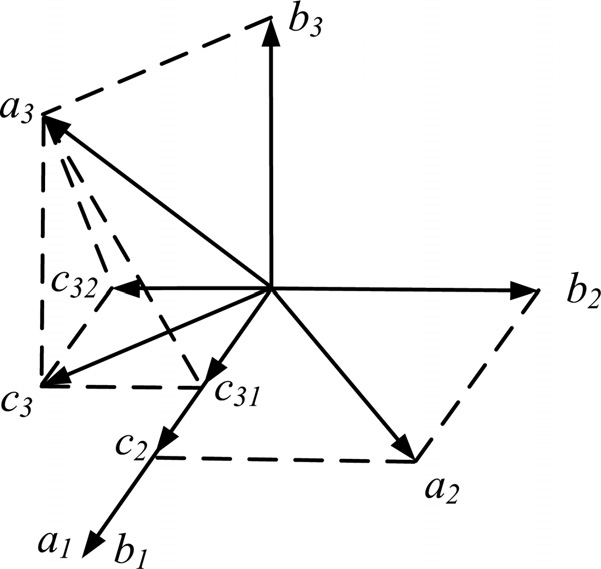
\includegraphics[width=0.25\textwidth]{An-illustration-of-Gram-Schmidt-transformation}
\end{figure}

To find all the vectors, we can write the following equations. For $r = 1, 2,
    \dots, n-1$ we have
\begin{equation}
    y_1 = x_1
\end{equation}
\begin{equation}
    y_{r+1} = x_{r+1} - \sum_{i=1}^{r}{\dfrac{\left(x_{r+1}, y_i\right)}{\left(y_i, y_i\right)}x_{r+1}}
\end{equation}

Or, alternatively
\begin{equation}
    y_{r+1} = x_{r+1} - \sum_{i=1}^{r}{\textnormal{proj}_{y_i}{x_{r+1}}}
\end{equation}

These are the formulas for \textbf{Gram-Schmidt} orthogonalization.

\begin{example}[Fourier Series]
    To approximate continuous functions in an interval $\left[0,2\pi\right]$, Fourier discovered that
    he could combine trigonometric polynomials. Let $V=C(0,2\pi)$ the linear space of all real continuous functions
    in the interval $\left[0,2\pi\right]$, we define the inner product as $\left(f,g\right) = \int_{a}^{b}{f(x)g(x)dx}$.

    Now, we try to find a normal set of trigonometric functions, this are the basis
    elements of our linear space. First, consider the functions $\cos{kx}$ and
    $\sin{kx}$. In a previous section we've seen that the norm of these functions
    is $\sqrt \pi$. Now, define a finite set of $n$ elements consisting of these
    trigonometric functions, and define them as $\psi_0, \psi_1, \dots$ where
    \begin{equation}
        \psi_0(x) = \dfrac{1}{\sqrt{2\pi}}, \quad \psi_{2k-1}(x) = \dfrac{\cos{kx}}{\sqrt{\pi}}, \quad \psi_{2k}(x) = \dfrac{\sin{kx}}{\sqrt{\pi}}
    \end{equation}

    for $k \geq 1$. You can check that $\left(\psi_{2k-1},
        \psi_{2k}\right)=\dfrac{1}{\pi}\int_{0}^{2\pi}{\cos{(kx)}\sin{(kx)}dx} = 0$ for
    all $k$. Also, for two elements $p,q\leq \dim V$ where $p\neq q$, we have that
    \begin{equation}
        \begin{split}
            \dfrac{1}{\pi}\int_{0}^{2\pi}{\cos(px)\cos(qx)dx} = 0 \\[1em]
            \dfrac{1}{\pi}\int_{0}^{2\pi}{\sin(px)\sin(qx)dx} = 0
        \end{split}
    \end{equation}

    Thus, the set $\Psi =
        \left\{\psi_0,\psi_1,\dots,\psi_{2k-1},\psi_{2k},\dots\right\}$ is a normalized
    orthogonal basis of $V$.

    These elements span a subspace $S$, so $S = L\left(\psi_0,\psi_1,\dots\right)$.
    If we want to approximate a function $f$, we must take the projection of $f$
    onto $S$. Let $f_n$ be the projection onto an $n$ dimensional subspace $S$
    spanned by the elements of $\Psi$:
    \begin{equation}
        f_n = \sum_{k=1}^{n}{(f, \psi_k)\psi_k}, \quad\textnormal{where }(f,\psi_k) = \int_{0}^{2\pi}{f(x)\psi_k(x)\,dx}
    \end{equation}
    Note that we omit the coefficient $\frac{1}{(\psi_k,\psi_k)}$, as $\psi_k$ is normalized it has norm $1$.

    Using the formulas in (3.23) we can write (3.25) as
    \begin{equation}
        f_n(x) = a_0 + \sum_{k=1}^{n}\left({a_k \cos{kx} + b_k \sin {kx}}\right)
    \end{equation}
    where
    \begin{equation}
        \begin{split}
            & a_0 = \dfrac{1}{2\pi}\int_{0}^{2\pi}{f(x)\,dx}        \\[1em]
            & a_k = \dfrac{1}{\pi}\int_{0}^{2\pi}{f(x)\cos(kx)\,dx} \\[1em]
            & b_k = \dfrac{1}{\pi}\int_{0}^{2\pi}{f(x)\sin(kx)\,dx}
        \end{split}
    \end{equation}

    \textbf{Fourier series} can be written as
    \begin{equation}
        f(x) = a_0 + \sum_{k=1}^{\infty}\left({a_k \cos{kx} + b_k \sin {kx}}\right)
    \end{equation}
\end{example}

\end{document}